\section{Prompt Robustness Details}
\label{app:robust}

\Tabref{tab:robust} lists the effect of each \CoT wording on the robustness subset (first 100 items of each task).
The 14B rows cover fewer items because the \cottwo run for that model did not finish (\secref{sec:robust}).

\begin{table}[h]
    \centering
    \caption{\CoT effect on the robustness subset for the main wording and the paraphrase, in accuracy points, with the 95\% bootstrap interval for the paraphrase (uncorrected). The 14B model has no logical-deduction items for \cottwo.}
    \label{tab:robust}
    \small
    \begin{tabular}{@{}llrrrc@{}}
        \toprule
        \textbf{Model} & \textbf{Category} & $n$ & \textbf{\cotc} & \textbf{\cottwo} & \textbf{\cottwo 95\% CI} \\
        \midrule
        0.5B & Pattern matching  & 200 & $-4.0$ & $-2.5$ & $[-5.0, -0.5]$ \\
             & Factual recall    & 200 & $-0.5$ & $-0.5$ & $[-6.0, +5.0]$ \\
             & Logical deduction & 200 & $+3.0$ & $+3.5$ & $[-5.0, +12.0]$ \\
             & Arithmetic        & 200 & $+50.0$ & $+58.0$ & $[+51.0, +65.0]$ \\
        \midrule
        1.5B & Pattern matching  & 200 & $-1.5$ & $-2.5$ & $[-5.0, -0.5]$ \\
             & Factual recall    & 200 & $+4.0$ & $-2.0$ & $[-7.5, +3.5]$ \\
             & Logical deduction & 200 & $+9.0$ & $+5.5$ & $[-3.0, +14.0]$ \\
             & Arithmetic        & 200 & $+76.0$ & $+75.5$ & $[+69.5, +81.0]$ \\
        \midrule
        3B   & Pattern matching  & 200 & $+1.5$ & $+3.5$ & $[+0.5, +7.0]$ \\
             & Factual recall    & 200 & $+4.0$ & $+3.5$ & $[-2.5, +9.5]$ \\
             & Logical deduction & 200 & $+15.0$ & $+16.5$ & $[+8.0, +25.0]$ \\
             & Arithmetic        & 200 & $+82.5$ & $+79.5$ & $[+74.0, +85.0]$ \\
        \midrule
        7B   & Pattern matching  & 200 & $-1.0$ & $0.0$ & $[-2.0, +2.0]$ \\
             & Factual recall    & 200 & $+4.5$ & $+3.0$ & $[-1.5, +7.5]$ \\
             & Logical deduction & 200 & $+27.0$ & $+24.0$ & $[+15.0, +33.0]$ \\
             & Arithmetic        & 200 & $+84.5$ & $+83.0$ & $[+77.5, +88.0]$ \\
        \midrule
        14B  & Pattern matching  & 178 & $-1.0$ & $-2.3$ & $[-4.7, -0.5]$ \\
             & Factual recall    & 175 & $+3.2$ & $-0.2$ & $[-4.0, +3.5]$ \\
             & Arithmetic        & 191 & $+80.3$ & $+76.6$ & $[+70.7, +82.2]$ \\
        \bottomrule
    \end{tabular}
\end{table}

\section{Per-Task Heatmap}
\label{app:heatmap}

\begin{figure}[h]
    \centering
    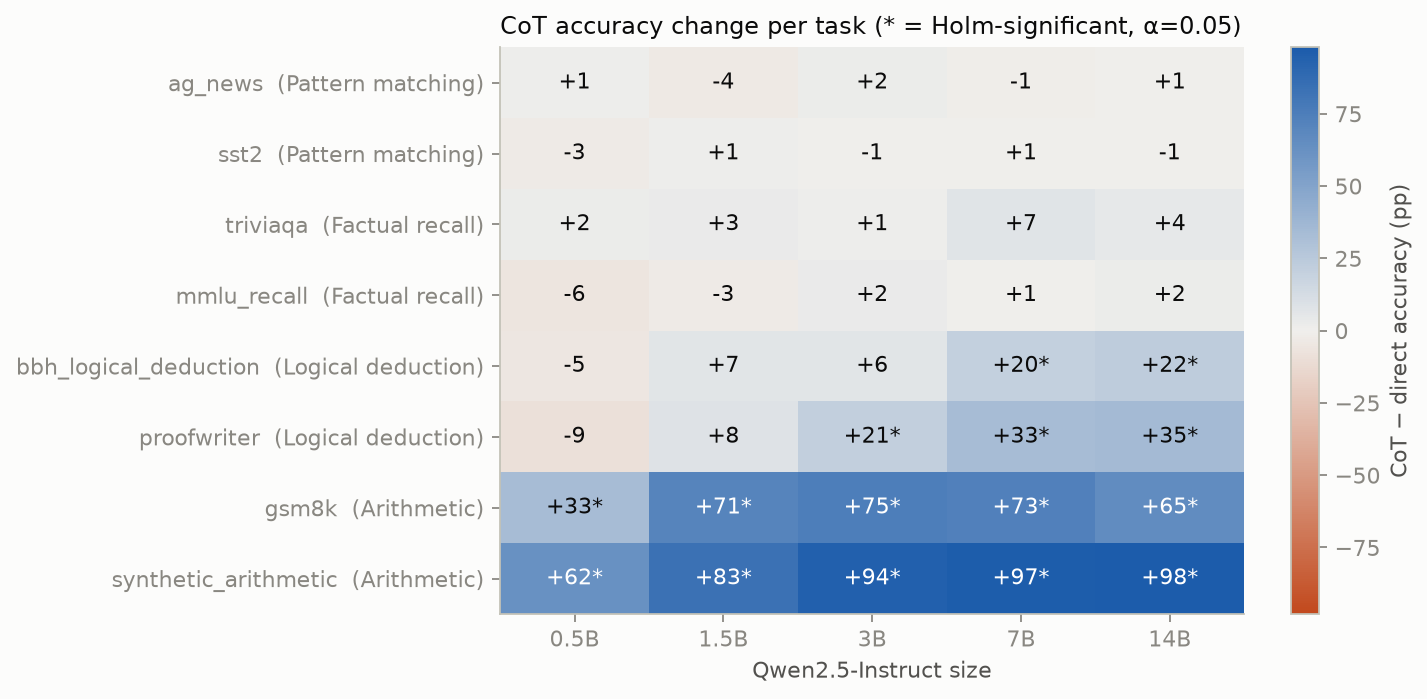
\includegraphics[width=0.8\linewidth]{figures/delta_heatmap.png}
    \caption{\CoT effect for every task and model size, in accuracy points. This is the same information as \tabref{tab:task}.}
    \label{fig:heatmap}
\end{figure}

\section{Compute and Implementation}
\label{app:compute}

We ran all models on four NVIDIA RTX A6000 GPUs (48 GB each) that were shared with other jobs, using Hugging Face \texttt{transformers} and PyTorch with bfloat16 weights.
Batch sizes were 64--96 and were halved automatically on out-of-memory errors.
The main grid took about 1 h 50 min of wall-clock time under contention; the 14B \CoT pass alone took about 55 min.
We sampled items with seed 42.
The analysis re-scores every response from the saved raw outputs.
